%! alt Isosceles triangle ABC with AB = AC and a 40 degree angle at A. Point D on side AC has BD = BC, with tick marks on BD and BC. The angles at B and C of triangle ABC are 70 degrees, angle DBC is 40 degrees, and the highlighted angle ABD is 30 degrees.
%! after_paragraph 1
%! scale 3/2
% The shared preamble of every Cevian figure. pipeline/figures turns these colours into theme-aware paint,
% and refuses any other colour, so draw only with them:
%   figink (lines and labels), figaux (construction lines), figaccent (the object the argument turns on),
%   figtint and figaccenttint (light fills).
\documentclass[border=1.5pt]{standalone}
\usepackage{tkz-euclide}
\definecolor{figink}{RGB}{0,0,0}
\definecolor{figaux}{RGB}{85,85,85}
\definecolor{figaccent}{RGB}{192,57,43}
\definecolor{figtint}{RGB}{221,221,221}
\definecolor{figaccenttint}{RGB}{245,213,208}
% tkz-euclide's defaults draw circles, compasses and marks in 50% grey and fill points with a tint.
\makeatletter
\def\tkz@otherlinecolor{figink}
\def\tkz@euc@circlecolor{figink}
\def\tkz@euc@compasscolor{figink}
\def\tkz@euc@mkcolor{figink}
\def\tkz@mk@fill{figink}
\def\tkz@euc@pointfillcolor{figink}
\makeatother
\tkzSetUpLine[color=figink,line width=.7pt]
\tkzSetUpArc[color=figink,line width=.7pt]
\tkzSetUpCompass[color=figink,line width=.5pt]
\tkzSetUpPoint[color=figink,fill=figink,size=3.1pt]
\tikzset{
  every picture/.style={line cap=round,line join=round,color=figink},
  circle style/.append style={color=figink,line width=.7pt},
  aux/.style={color=figaux,line width=.45pt,dash pattern=on 2.6pt off 2pt},
  key/.style={color=figaccent,line width=1pt},
  mk/.style={color=figink,line width=.5pt},
  lbl/.style={color=figink,inner sep=2.2pt},
  len/.style={color=figink,inner sep=1.5pt,font=\small},
}

\begin{document}
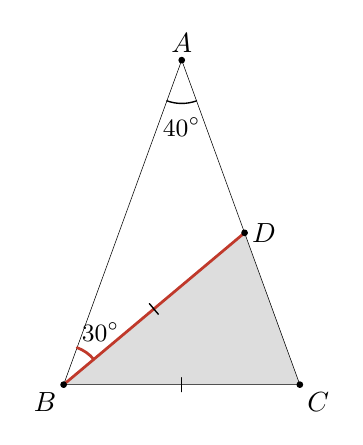
\begin{tikzpicture}
\tkzDefPoint(0.0,0.0){B} %! B = (0, 0)
\tkzDefPoint(3.0000000,0.0){C} %! C = (2, 0)
\tkzDefPoint(1.5000000,4.1212161){A} %! A = (1, 1/tand(20))
\tkzDefPoint(2.2981333,1.9283628){D} %! D = polar(B, 2, 40)
%! fact equal(dist(A, B), dist(A, C))
%! fact angle(B, A, C) == 40
%! fact on_segment(D, A, C)
%! fact equal(dist(B, D), dist(B, C))
%! fact angle(D, B, C) == 40
%! fact angle(A, B, D) == 30
\tkzFillPolygon[color=figtint](B,C,D)
\tkzDrawPolygon(A,B,C)
\tkzDrawSegment[key](B,D)
\tkzMarkSegments[mark=|,size=2.5pt,mk](B,D B,C)
\tkzMarkAngle[size=.55,arc=l,mark=none,mk](B,A,C)
\tkzMarkAngle[size=.5,arc=l,mark=none,key](D,B,A)
\tkzLabelAngle[pos=.85,font=\small](B,A,C){$40^\circ$}
\tkzLabelAngle[pos=.82,font=\small](D,B,A){$30^\circ$}
\tkzDrawPoints(A,B,C,D)
\tkzLabelPoint[above,lbl](A){$A$}
\tkzLabelPoint[below left,lbl](B){$B$}
\tkzLabelPoint[below right,lbl](C){$C$}
\tkzLabelPoint[right,lbl](D){$D$}
\end{tikzpicture}
\end{document}
